\documentclass{article}
\usepackage[utf8]{inputenc}
\usepackage{graphicx}

\title{Contrastive Fusion with Knowledge Graph for Semantic Product Search}

\author{Authors}
\date{June 2022}

\begin{document}

\maketitle

\begin{abstract}
How to fuse negative knowledge?
\end{abstract}

\section{Introduction}

Semantic product search is an essential task in e-commerce. In such scenario, the length of the text is usually short and contains less information, which can easily cause model misunderstanding. Thus, domain knowledge plays an important role. For instance, in search scenario, due to the lack of the knowledge that ``Sunshine Rose'' is a grape variety, ``rose'' and ``Sunshine Rose grape'' will be easily misjudged as highly correlated. Besides, some text pairs are textually similar but not semantically relevant, such as ``green orange'' and ``green apple''. Such kind of problem can be effectively solved by fusing knowledge into the model. 

Nowadays, e-commerce platforms are committed to constructing commodity knowledge graphs, which can be a good source of knowledge. Then, how to effectively make use of knowledge graph to assist semantic product search task is a question that worth delving into. Figure 1 is a general framework for most knowledge graphs in e-commerce scenario. There are mainly two components in the knowledge graph: a coarse-grained taxonomy and a set of fine-grained e-commerce concepts. The coarse-grained taxonomy is usually manually constructed to organize products in a coarse-grained manner. The nodes in the taxonomy is connected by isA relationship .To better meet user need, a set of fine-grained e-commerce concepts is usually constructed automatically or semi-automatically. The concepts are usually mined from large corpora in e-commerce, such as search queries, product titles, user-written reviews, etc.[Alicoco] In the e-commerce concepts set, there is also synonym relationship apart from isA relationship. Products and queries can be linked to the knowledge graph. 

\begin{figure}[h]
    \centering
    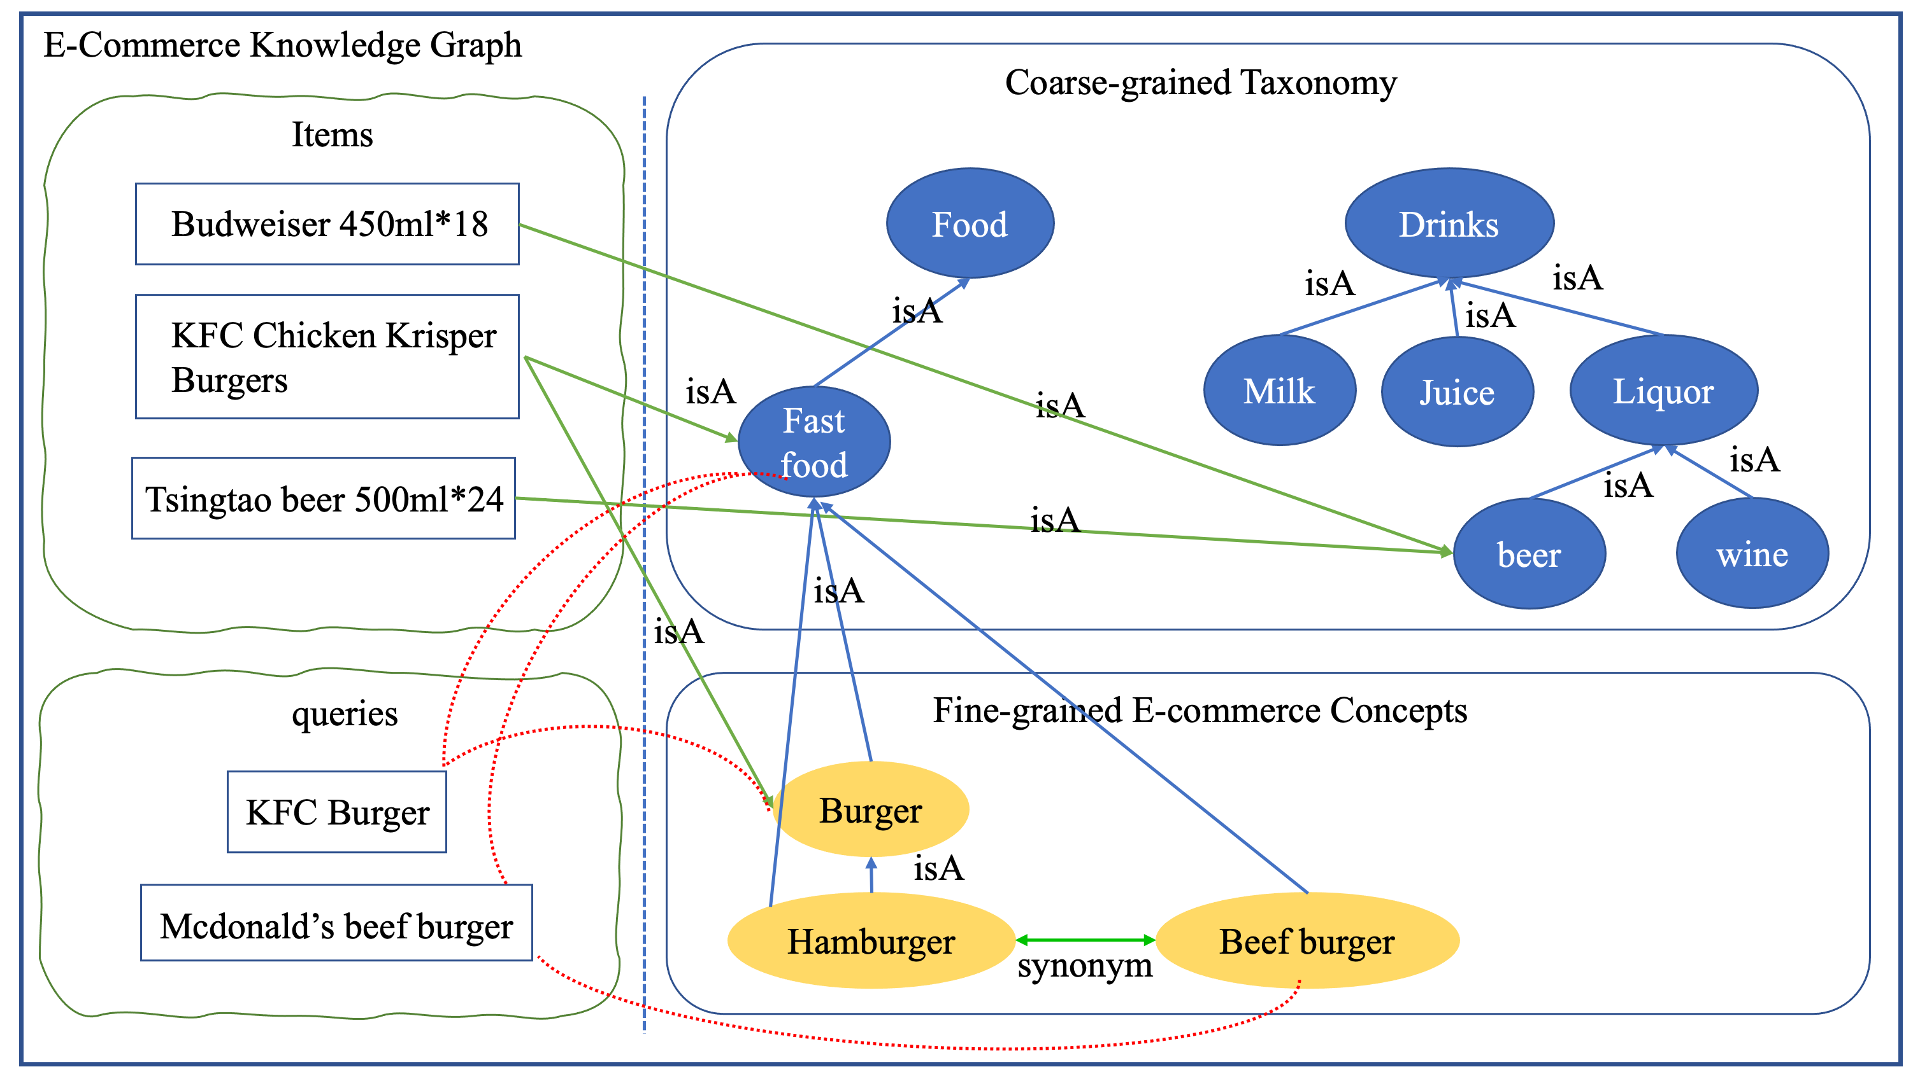
\includegraphics[scale=0.4]{mtkg.png}
    \caption{General knowledge graph framework in e-commerce}
    \label{fig2}
\end{figure}

Currently, there are three main solutions to implement knowledge fusion: (1) Pre-training-based method (2) data augmentation-based method and (3) Online knowledge fusion method. \textbf{Pre-training-based method} does knowledge fusion in the pre-training stage by designing relevant joint-training tasks. After pre-training, the model will be fine-tuned for downstream tasks. However, because of the difference of data and objective in two stages, it is difficult to transferred the knowledge fused during pre-training stage to downstream tasks. \textbf{Data augmentation-based method} aims to improve generalization ability of models by constructing more data samples in training set using knowledge graph. Through augmenting more samples from knowledge graph, model can learn more knowledge and be more intelligent. However, in order to fuse knowledge as much as possible, we have to construct text pairs by enumeration, which is labor expensive and makes training set redundant. Besides, there will inevitably be noisy samples in the augmented data set, and it may mislead model. Data augmentation will also make the data distribution different from the original distribution. \textbf{Online knowledge fusion method} fuse retrieved relevant knowledge of samples from knowledge graph to original samples. This method can effectively fuse positive knowledge to the model. For example, it can help model learn that "Sunshine Rose" is a grape variety by adding category information. The problem of this method is that it cannot effectively fuse negative knowledge, so it lacks the ability to distinguish textually similar but semantically irrelevant text pairs. 


Our contributions are as follows:
\begin{itemize}
\item[$\bullet$] Open source data set. We release a Chinese data set for semantic product search task, so that it would be more convenient for other researchers to provide better solutions. 
\item[$\bullet$] Comparison analysis of different knowledge fusion methods for semantic product search task. We analyze different knowledge fusion methods for the task and identify main challenges of this task and problems of current knowledge fusion methods.
\item[$\bullet$] Contrastive Knowledge fusion framework. We propose a novel knowledge fusion framework ... 
\end{itemize}


\section{Background}

\section{Problem Definition}

\subsection{Semantic Product Search}

For the semantic product search task, we clarify it as follows. Given a set $ S $ of $ n $ text pairs,

$ \{<A_{1},B_{1}>,<A_{2},B_{2}>, ... ,<A_{n},B_{n}>\} $

each pairs consists of two terms, $A_{i}$ and $B_{i}$.  $A_{i}$ is user query and $B_{i}$ is the title of product. The goal of this task is to compute the relatedness of each pair. 
\subsection{Knowledge Graph}

In order to explore the effectiveness of different knowledge fusion methods, knowledge graph $G=\{V,E\}$ is the source of knowledge for the problem in this paper. $V$ is a set of e-commerce concept nodes and $E$ is a set of relationships.


\section{Approach}
In this section, we propose a general way to  novel method to calculate the relatedness between query and product based on knowledge graph.
\subsection{Method Introduction}
\subsubsection{Contrastive Task}
Construct positive and negative samples based on two-hop relationship from query or product to graph nodes (query/product→node→query/product).

\subsubsection{Multitask learning}
2 contrastive loss + 1 CE loss.

\subsection{Pseudo knowledge graph construction}
    \subsubsection{Query Graph Construction}
    \subsubsection{Product Graph Construction}


\section{Experiment}
\subsection{Experiments of Open Sourced Data Set}

\subsection{Comparison with other Knowledge Fusion Methods}

\begin{center}
\begin{tabular}{lc}
   \toprule
   \textbf{Method} & \textbf{Metrics}  \\
   \midrule
   Sentence-BERT & none  \\
   ConSERT & none  \\
   SimCSE & none  \\
   Sentence-BERT_{str-cat} & none  \\
   Pre-train based method & none  \\
   Graph learning method & none  \\
   Ours & none \\
   \bottomrule
\end{tabular}
\end{center}
\subsection{Noise Knowledge Robustness Experiment}

\subsection{Ablation Study}
\begin{center}
\begin{tabular}{lc}
    \toprule
    Choice & metrics \\    
    \midrule   
    Sentence-BERT & metrics \\
    Sentence-BERT w/ query cont & metrics \\
    Sentence-BERT w/ doc cont  & metrics \\
     Sentence-BERT w/ all  & metrics \\
    \bottomrule
\end{tabular}  
\end{center}

\subsection{Visualization}

\section{Related Work}
\section{Conclusion}
\section{References}
\
\end{document}
